\documentclass[a4paper,10pt]{article}
\usepackage[utf8]{inputenc}
\usepackage{amsmath}
\usepackage{multirow}
\usepackage{amssymb}
\usepackage{graphics}
\usepackage{hyperref}
\usepackage{placeins}
\usepackage{caption}
\usepackage{subcaption}
\usepackage[normalem]{ulem}

\usepackage{amssymb}

\usepackage{graphicx}
\usepackage[outdir=./]{epstopdf}

\usepackage{cite}

% \renewcommand\topfraction{0.85}
% \renewcommand\bottomfraction{0.85}
% \renewcommand\floatpagefraction{0.85}

\usepackage{float}

\usepackage{tikz}


\usepackage{todonotes}


% \usepackage[lined,boxed]{algorithm2e}
\usepackage[linesnumbered,ruled]{algorithm2e}
\SetStartEndCondition{ (}{)}{)}\SetAlgoBlockMarkers{\{}{\}}%
\SetKwProg{Fn}{}{}{}\SetKwFunction{FRecurs}{void FnRecursive}%
\SetKwFor{For}{for}{}{}%
\SetKwIF{If}{ElseIf}{Else}{if}{}{elif}{else}{}%
\SetKwFor{While}{while}{}{}%
\SetKwRepeat{Repeat}{repeat}{until}%
\AlgoDisplayBlockMarkers\SetAlgoNoLine%

\usepackage{geometry}
 \geometry{
 a4paper,
 total={150mm,257mm},
 left=30mm,
 top=40mm,
 bottom=40mm,
 }

\setlength{\parindent}{0ex}
\setlength{\parskip}{1em}

\usepackage{tikz}
\usetikzlibrary{3d,calc}
\usetikzlibrary{arrows, decorations.markings}
\tikzstyle{vecArrow} = [thick, decoration={markings,mark=at position
   1 with {\arrow[semithick]{open triangle 60}}},
   double distance=1.4pt, shorten >= 5.5pt,
   preaction = {decorate},
   postaction = {draw,line width=1.4pt, white,shorten >= 4.5pt}]



\title{Boundary Integral Equations - Project \\ Nearly Singular Integrals and Special Quadrature}
\author{Fredrik Fryklund and Sara P\aa lsson}

\begin{document}

\maketitle

\section*{Introduction}
This project deals with the optimization and parallelization of solving linear equations with boundary integral equation (BIE) methods. To demonstrate the strengths and weaknesses with a BIE method, and how to make the computations for these faster, we use the example problem of solving Laplace's equation in two-dimensions on a starfish domain. Therefore, before going  into details on our existing code, performance analysis and parallelization, we start by overviewing the methods we will use. 

\subsection*{Boundary Integral Equations}
Boundary integral equations (BIE) provide a way to solve linear equations to a high accuracy. By reformulating the differential equation as an integral equation over the surface of our domain, we reduce the degrees of freedom of the problem compared to a standard grid-based method where we discretize the whole domain, for example finite element and finite difference methods. A simple sketch of the differences between a standard grid-based method and a BIE method can be seen in Fig. \ref{fig:disc}, where we have used squared elements for our standard grid and discretized the BIE with equidistant points along the boundary. Here, show the discretization for a starfish domain in two dimensions, which is smooth. This is going to be our example domain throughout this report. 
\begin{figure}[ht]
	\begin{center}
		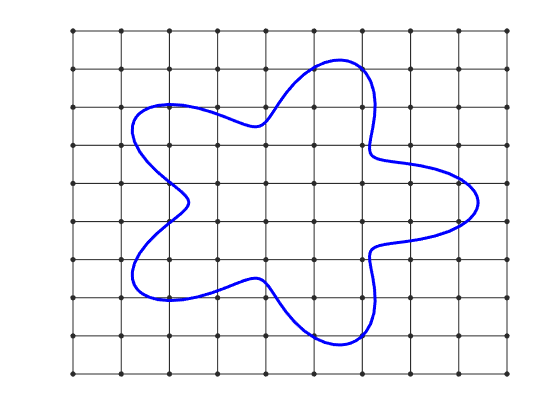
\includegraphics[width=0.45\textwidth]{Graphics/starfish_grid.png}
		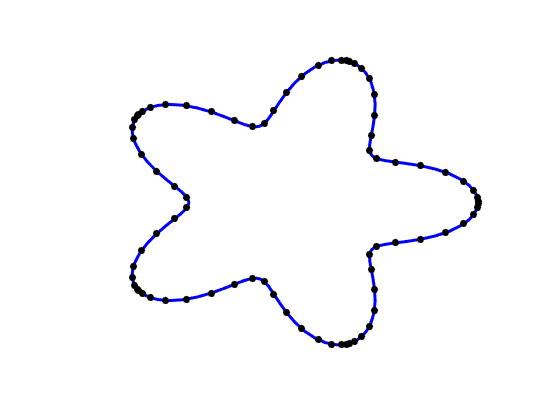
\includegraphics[width =0.45\textwidth]{Graphics/starfish_BIE.png}
	\end{center}
	\caption{Typical examples of grid-based discretization (left) and BIE discretization (right) of a starfish domain.}
	\label{fig:disc}
\end{figure}
\\ \\
For completeness, we state Laplaces equation in our domain $\Omega\in\mathbb{C}$, 
\begin{align}
	\begin{split}
		\Delta u = 0, \; z\in\Omega, \\
		u(z) = f(z), \; z\in\delta\Omega,  
	\end{split}
	\label{eq:laplace}
\end{align}
with the analytic function $f(z)=\frac{1}{z-z_1}+\frac{1}{z-z_2} + \frac{1}{z-z_3}$, $z_1,\,z_2,\,z_3\,\notin\Omega$, as boundary condition. As $f$ is analytic, the solution to \eqref{eq:laplace} is known as $u(z)=f(z)$ for all $z\in\Omega$. This provides us with an easy way to check the errors from our different quadrature schemes. For a boundary integral method, solving \eqref{eq:laplace} means to first compute the complex density $\mu(z)$ for all $z\in\delta\Omega$ through
\begin{align}
	\frac{1}{2}\mu(z) + \frac{1}{2\pi}\int_{\delta\Omega} \mu(\tau) \Im\left\{ \frac{d\tau}{\tau-z}\right\} = f(z).
	\label{eq:density}
\end{align}
For the points $z = \tau$ on the boundary, we have the limit 
\begin{align*}
\lim_{z\rightarrow\tau} \Im\left\{ \frac{\tau^\prime}{\tau-z}\right\} ) = \Im\left\{ \frac{\tau^{\prime\prime}}{\tau-z} \right\}.
\end{align*}
When we have computed $\mu$, we can compute the solution $u(z)$ at all points $z$ both on the domain and in the boundary, through
\begin{align}
	u(z) = \frac{1}{2\pi} \int_{\delta\Omega} \mu(\tau) \Im\left\{ \frac{d\tau}{\tau-z} \right\}.
\label{eq:ulapl}
\end{align}
There are several advantages with a boundary discretization: the reduction of degrees of freedom means we will have a smaller system to solve in \eqref{eq:density}, we know the position of the interface explicitly and do not need to interpolate from a domain-based grid, and we can easily track movement of the interface. Other methods for tracking interfaces, such as immersed boundary methods, perform only to low orders of accuracy, whilst we with a BIE obtain spectral accuracy. The accuracy of a BIE method is decided by the quadrature, and if we use  a high-order quadrature method to evaluate our integrals our method will be of high order. There are of course also drawbacks with this kind of methods. Firstly, the system we need to solve to compute $\mu$ in \eqref{eq:density} is dense (albeit smaller than that of a grid-based scheme due to the decrease in degrees of freedom). However, algorithms such as \textit{gmres} still converge quickly, as our condition numbers are more or less constant and also small. 
\\ \\
As mentioned previosuly, the integrals we evaluate will contain singularities. These do not pose any problem, as we can use known limits or singularity subtraction to handle such cases. However, as we evaluate our integral in \eqref{eq:ulapl} close to the boundary of our domain, the integral will become so-called ``nearly singular''. This means that whilst the integrand mathematically is smooth and well-defined, numerically it will be difficult to resolve and our errors will increase dramatically. To see this specifically, we look at the integrand
\begin{align}
k(\tau,z) = \Im\left\{ \frac{\tau^\prime}{\tau-z}\right\}.
\label{eq:kernel}
\end{align}
As $z$ becomes closer and closer to $\tau$, this will give us a denominator that is approaching zero, and the integrand will therefore grow rapidly. This will be increasingly difficult to resolve, and simply upsampling the discretization on the boundary $\delta\Omega$ will not be sufficient. For these cases, we need to do something different and will apply a special quadrature.
\\ \\
A short summation of the special quadrature follows. For a more detailed description, see \cite{ojalahelsing}. When it comes to solving \eqref{eq:ulapl} with special quadrature, we use the fact that the kernel \eqref{eq:kernel} is the same as in the monomials 
\begin{align}
    p_k(z) = \int \frac{\tau^k}{\tau-z}d\tau, \; k=0,\hdots,31.
    \label{eq:pkrec}
\end{align}
For $p_0(z)$ we have the analytical solution 
\begin{align}
    p_0(z) = \log(1-z)-\log(-1-z).
    \label{eq:p0}  
\end{align}
The other $p_k$ can be obtained through a simple recursion. Thus, for a panel $P_j$ we can write
\begin{align}
    \int_{P_j} \mu(\tau) \Im\left\{ \frac{d\tau}{\tau-z} \right\} = \Im\left\{ \sum_{k=0}^{31} c_k \int_{P_j} \tau^k\frac{d\tau}{\tau-z} \right\} = \Im\left\{ \sum_{k=0}^{31} c_kp_k \right\},
    \label{eq:specQ}
\end{align}
where $\mu_j(z) = \sum_{k=0}^{31} c_k\tau^k$ is the polynomial interpolation of $\mu$ restricted to panel $P_j$. 
\\ \\
As a demonstration for how the special quadrature works, we show in Fig. \ref{fig:normquad} how the error in $u$ behaves as we approach the boundary $\delta\Omega$. The number of panels influences the error, but as can be seen upsampling does not completely remove the problems. In comparison, in Fig. \ref{fig:specquad} we see the error after applying the special quadrature. Also for 35 panels, the errors are negligble. 
\begin{figure}[ht]
    \begin{center}
        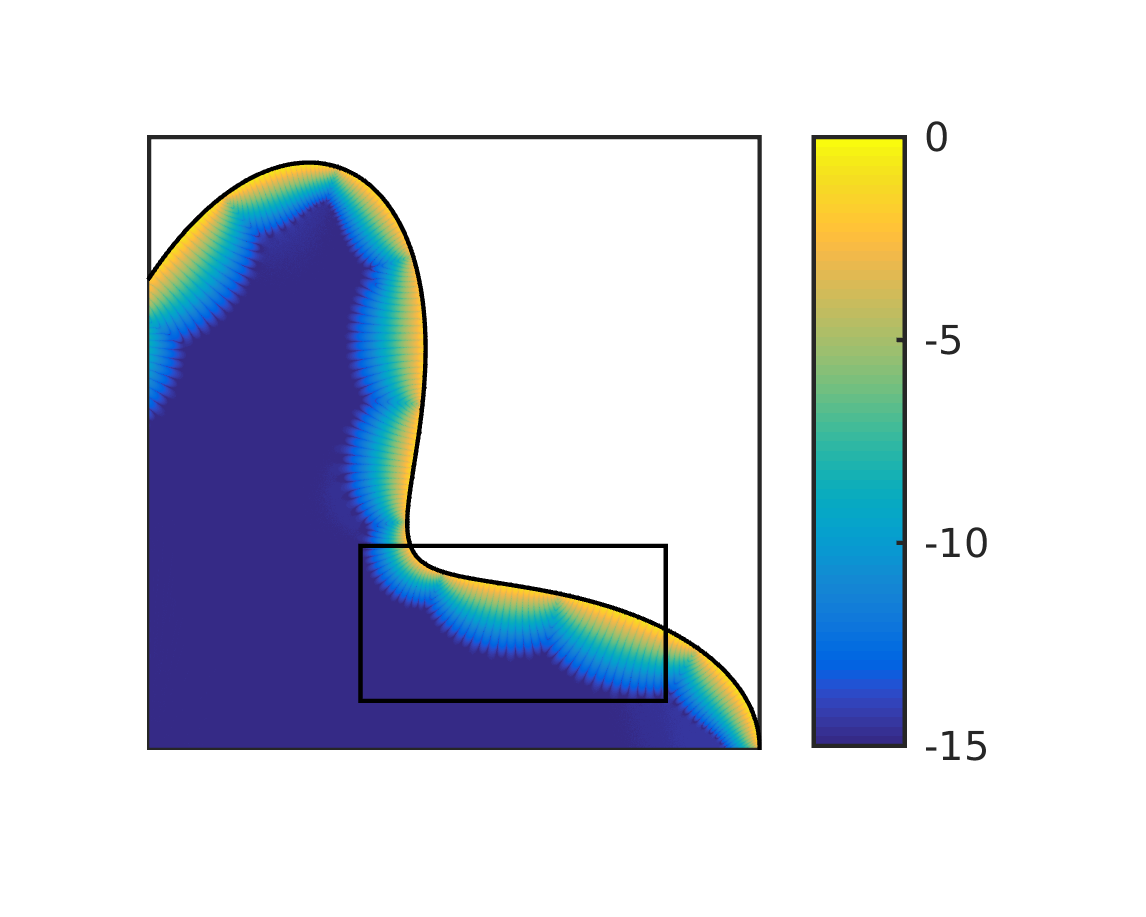
\includegraphics[width=0.49\textwidth]{Graphics/filled_error_panels35.png}
        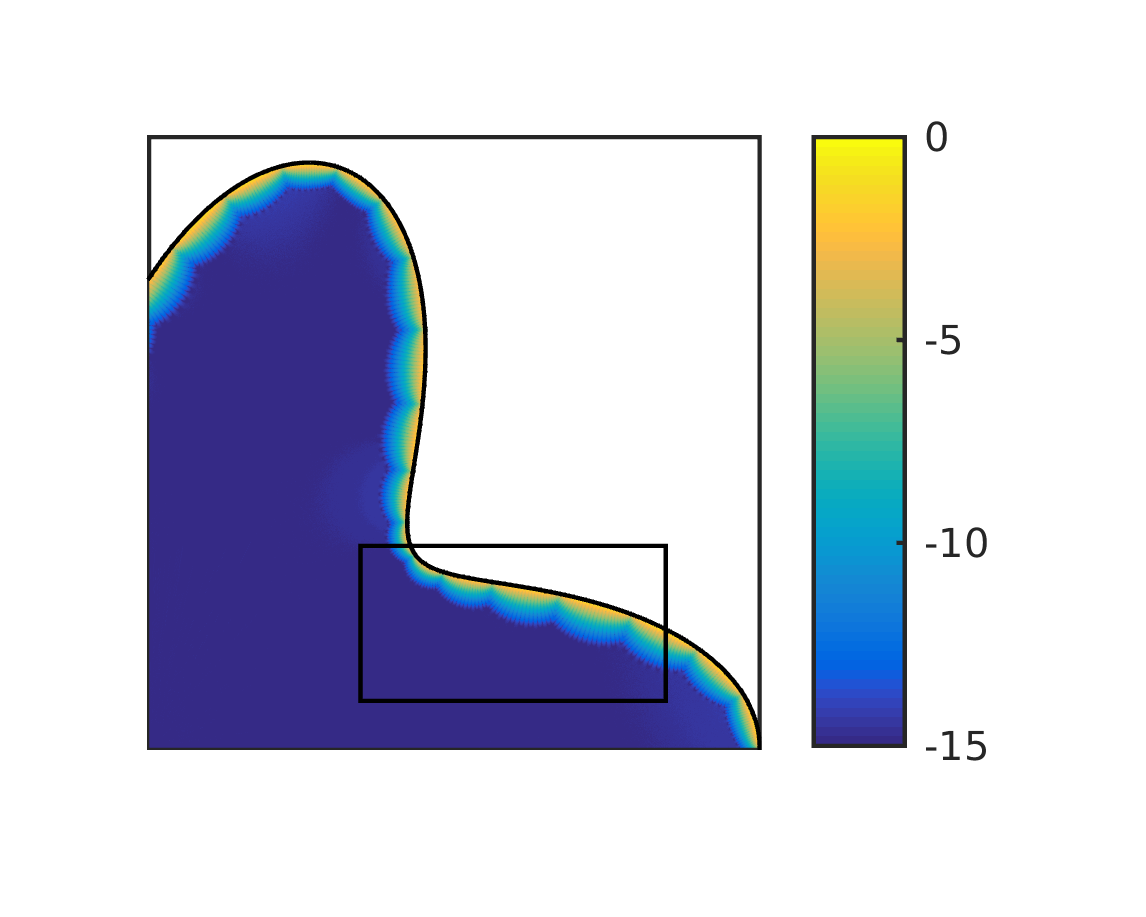
\includegraphics[width =0.49\textwidth]{Graphics/filled_error_panels70.png}
    \end{center}
    \caption{Example of error in domain when solving Laplace's equation, using only normal quadrature, using 35 panels (left) and 70 panels (right).}
    \label{fig:normquad}
\end{figure}
\begin{figure}[ht]
    \begin{center}
        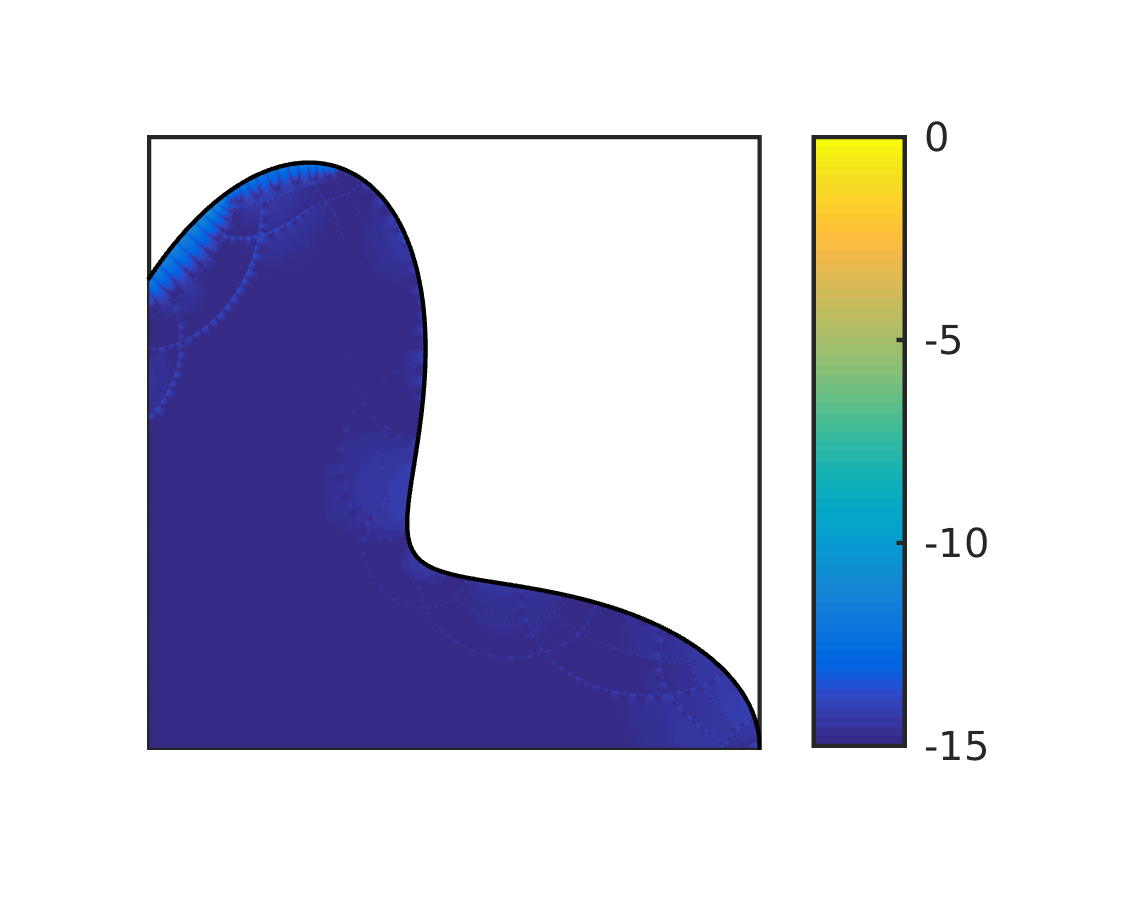
\includegraphics[width=0.49\textwidth]{Graphics/fillederror_SQ_panels35.png}
        \end{center}
    \caption{Error after application of special quadrature, for 35 panels.}
    \label{fig:specquad}
\end{figure}
If we zoom in and compare the level curves for the error in the black box, we see that the special quadrature removes all errors up to $\approx 10^{-15}$, see Fig. \ref{fig:levelcurves}. 
\begin{figure}[ht]
    \begin{center}
        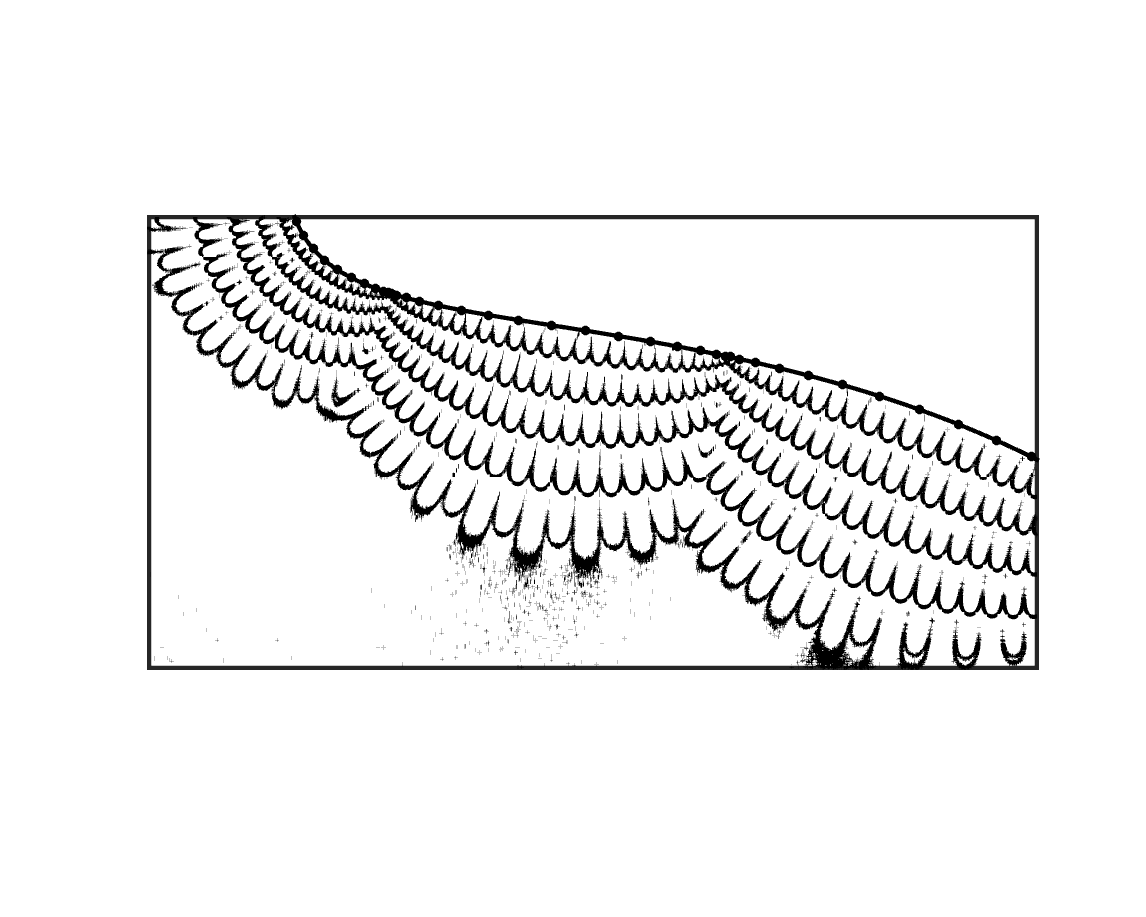
\includegraphics[width=0.49\textwidth]{Graphics/contour_panels35.png}
        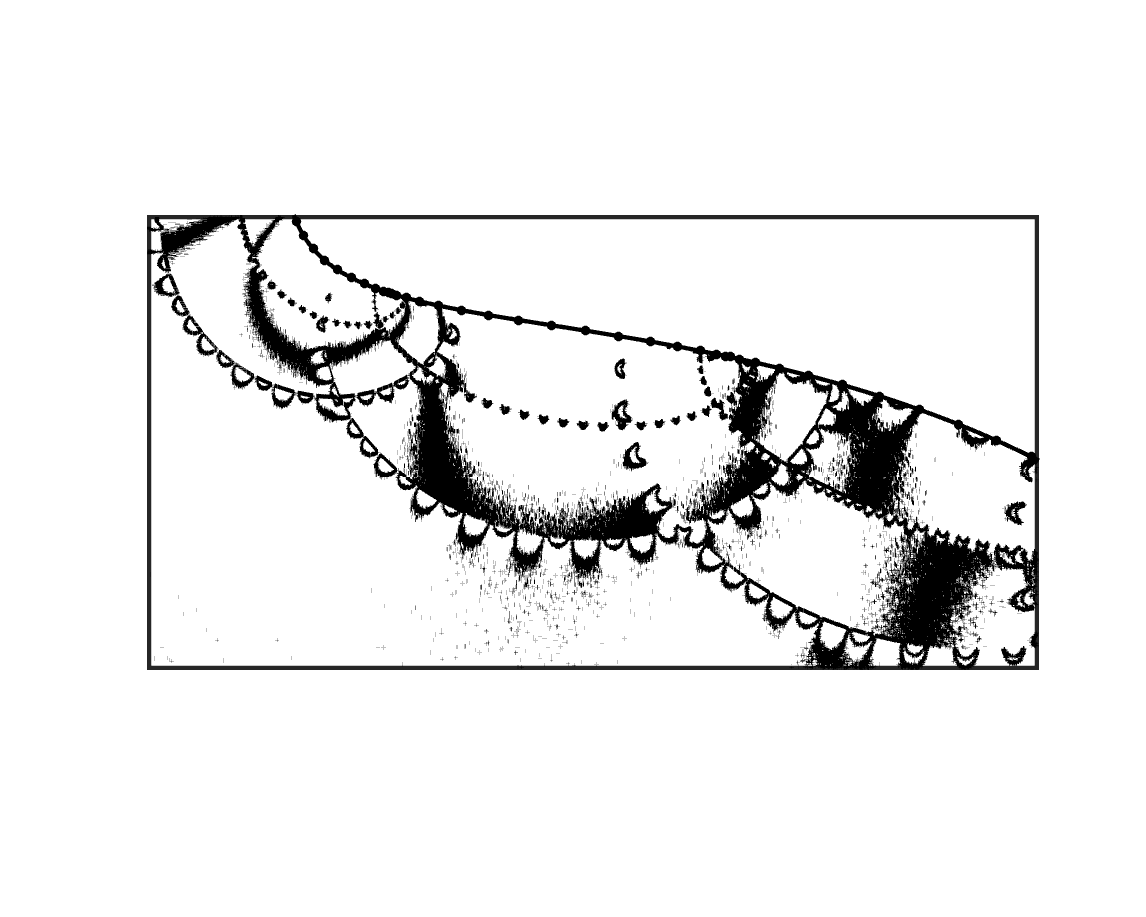
\includegraphics[width =0.49\textwidth]{Graphics/contour_SQ_panels35.png}
    \end{center}
    \caption{Error curves, for normal quadrature, $\log_{10} e(z) = \{ -15,-12,-9,-6, -3 \}$ (left) and special quadrature (only $\log_{10} e(z) = -15$ visible) (right).}
    \label{fig:levelcurves}
\end{figure}
\FloatBarrier

\section*{The Algorithm}
The algorithm to compute the boundary integral solution is divided up into several parts. The three major ones are to compute the complex density $\mu$ through \eqref{eq:density}, compute the solution $u$ everywhere in the domain through \eqref{eq:ulapl} and finally to compute corrections to $u$ using special quadrature in those cases it is needed. When discretizing our boundary $\delta\Omega$, we divide it into panels on which we put 16 Gauss-Legendre nodes each. The domain is discretized radially and angularly, going from the middle outwords towards $\delta\Omega$ anti-clockwise. Here, we describe each algorithm briefly. The algorithms can be found in Appendix \ref{sec:alg}. 
\\ \\
First, in Alg. \ref{alg:solveDensity} we solve \eqref{eq:density} for the complex density $\mu$. This is done by first filling the system matrix $A$, through two \textit{for}-loops. We then compute $\mu$ through \textit{gmres}. Our matrix $A$ is dense and real-valued, but not symmetric. The major parts of the algorithm are thus two for-loops of the \textbf{boundary} discretization points, and a call to \textit{gmres}.
\\ \\
The next step is to compute the solution in the domain through \eqref{eq:ulapl}. We do this by integrating our $\mu$ over the boundary $\delta\Omega$, using the same discretization as in Alg. \ref{alg:solveDensity}. This becomes one for-loop over the \textbf{domain} discretization points and one over the \textbf{boundary} discretization points (typically fewer than those on the boundary), see Alg. \ref{alg:compU}.
\\ \\
The final major step of the algorithm is to apply the special quadrature \cite{ojalahelsing} to reduce the errors in $u$ close to the boundary. This algorithm is briefly described in Alg. \ref{alg:specQ}. It consists of a for-loop over all domain points $\tau_i$, and then a for-loop over all panels of the domain discretization $P_j$. For each panel and point pair, the distance between them is computed. If the distance is less than a set threshold, further investigations are needed. We will compute an analytical and numerical value of $p_0$ \eqref{eq:p0}, which contains the same kernel as our solution integral. If these two values of $p_0$ differ by less than a constant, our integral is deemed well resolved. If not, we upsample to 32 points Gauss-Legendre quadrature on the panel, and compare $p_0$ again. Now, if the upsampled integral gives a good value of $p_0$ we assume that also our integral for $u_i$ will be well resolved for point $\tau_i$ on panel $P_j$. We therefore compute a new value for $u_i$ on $P_j$ only, and add it to $u_i$. If upsampling is not enough, we apply our special quadrature. We then need to compute all $p_k$ through a recursion, \eqref{eq:pkrec}, and then find the coefficient to interpolate this to a polynomial of degree 15. This is done through solving a Vandermonde system. We then compute our new value of $u_i$ on panel $P_j$ with the specal quadrature \eqref{eq:specQ}. 
\FloatBarrier

\section*{Performance of Serial Code}
We analyze our code using CrayPAT as well as a function to time the separate functions individually without CrayPAT (convenient when making several runs). We test both the dependency on the number of panels $N_{pan}$ as well as the number of discretization points $N_{dom}$.

\subsection*{Changing Domain Discretization}
Firstly, we investigate how our code changes as we change the number of domain points, $N_{dom}$. In these tests, we have set $N_{pan}=20$ which gives us an error of $\approx 10^{-8}$. For some different $N_{dom}$ ranging from $25$ to $13$ million we see the timings in Fig. \ref{fig:serial1}. For small $N_{dom}$, the total computation time is dominated by the time it takes to solve the linear system when computing the complex density $\mu$. For this example that cost will be constant as we keep $N_{pan}$ constant, and $\mu$ is independent of the domain discretization points. As $N_{dom}$ grows, the cost will be dominated by the computation of $u$ with standard quadrature and the special quadrature. They both show the same cost, which is natural as the main feature of both algorithms is a for-loop through all points. We can also see this as they show complexity $O(N)$, which a for-loop would. 
\begin{figure}[ht]
    \begin{center}
        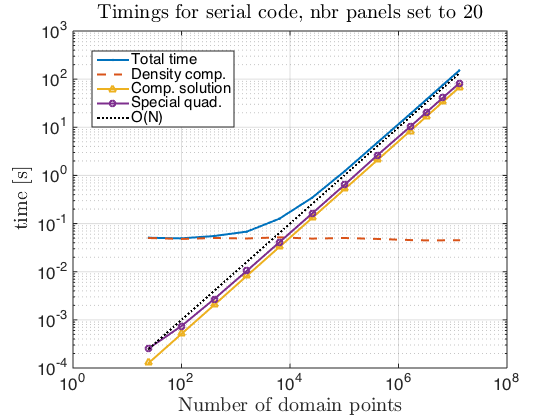
\includegraphics[width=0.8\textwidth]{Graphics/timing_serial_npanels20.png}
    \end{center}
    \caption{Timings serial code for varying $N_{dom}$. Fixed $N_{pan}=20$.}
    \label{fig:serial1}
\end{figure}

\subsubsection*{Performance Analysis}
Next, we investigate the code with CrayPAT as we change $N_{dom}$. We start by studying a problem were we are still using a relative small amount of points in our domain, i.e. were \textit{solveDensity}, Alg. \ref{alg:solveDensity}, dominates the cost. This problem is run for $N_{dom} = 1600$, $N_{pan}=20$. When studying the performance through CrayPAT, we see that the call to \textit{gmres} takes most time, see Fig. \ref{fig:batch4_serial_pie}. We set that the functions being called the most times, such as \textit{IPMultR} and \textit{tau} e.g., are very quick, whereas the three major algorithms pin-pointed earlier indeed take the most time. We see in the right pie chart, that it is the \textit{gmres}-call that takes up the most time. 
\begin{figure}[ht]
    \begin{center}
        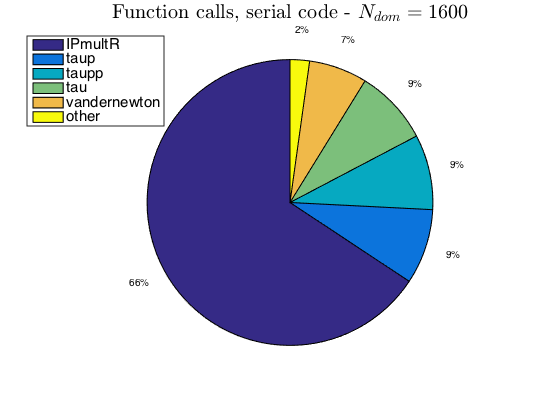
\includegraphics[width=0.49\textwidth]{Graphics/craypat_serial_batch4_calls_pie.png}
        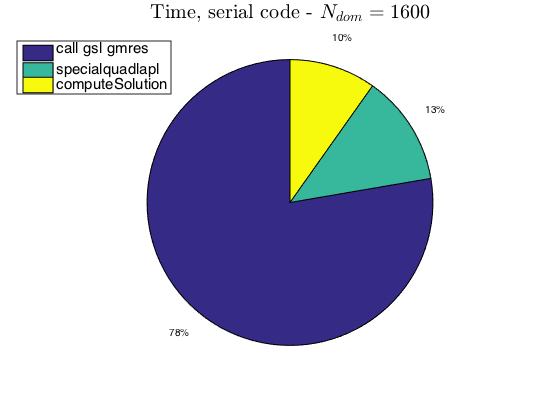
\includegraphics[width=0.49\textwidth]{Graphics/craypat_serial_batch4_time_pie.png}
    \end{center}
    \caption{Number of function calls and times for serial code $N_{dom} = 1600$, $N_{pan} = 20$.}
    \label{fig:batch4_serial_pie}
\end{figure}
Furthermore, if we investigate (USER) cache misses, we see that our code has a quite bad hit/miss ratio, see Tab. \ref{tab:batch4_serial_caches}. Our total D1 cache hit/miss ratio, however, seem to be decreased by the function call to \textit{call\_gsl\_gmres}, which is the \textit{gmres} solver in the GSL-package. Other bad results worth noticing and investigating further, seem to be the poor D2 hit/miss ratio by \textit{computeSolution}. 
\begin{table}[ht]
\begin{center}
    \begin{tabular}{ c | c | c | c | c }
        Function & D1 hit/miss (\%/\%) & D2 hit/miss & D1+D2 hit/miss & Time (\%) \\ \hline
        Total & $47.9/52.1$ & $28.3/71.7$ & $62.7/37.3$ & $100$ \\ 
        call\_gsl\_gmres & $23.5/76.5$ & $31.4/68.6$ & $47.5/52.5$ & $70.9$ \\
        specialquadlapl & $97,8/2.2$ & $100/0$ & $100/0$ & $11.4$ \\
        computeSolution & $100/0$ & $0/100$ & $38.1/61.9$ & $8.9$ \\
        gl16 & $98.5/1.5$ & $14.2/85.8$ & $79.82/9.98$ & $2.7$ \\
        vandernewton & $99.8/0.2$ & $100/0$ & $100/0$ & $2.6$ \\
        solveDensity & $99.8/0.2$ & $51.3/48.7$ & $99.9/0.1$ & $2.5$
    \end{tabular}
    \caption{D1 and D2 cache hit and miss ratios for serial code, $N_{dom} = 1600$. Data generated by CrayPAT.}
    \label{tab:batch4_serial_caches}
\end{center}
\end{table}  \\
Now, we study the timings and cache missed for a problem with larger $N_{dom}$, i.e. when those computations dominates over the panel computations. We set $N_{dom} = 3276800$ and keep, as before, $N_{pan}=20$. In Fig. \ref{fig:batch10_serial_pie} (left) we see that the number of function calls is dominated, still, by \textit{IPmultR} and \textit{vandernewton}. The functions \textit{tau, taup, taupp} no longer influence the computations as they are called only once in the beginning of the simulation, to set up the boundary domain. Regarding the time consumption, it is now clear (right figure) that the call to \textit{gmres} is no longer of any significance. Now the computation is dominated instead by \textit{specquadlapl} and \textit{computeSolution}.
\begin{figure}[ht]
    \begin{center}
        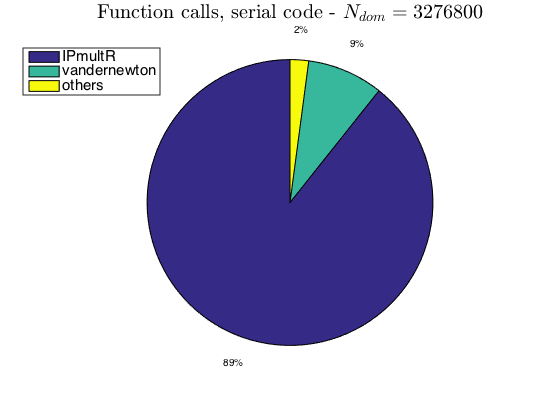
\includegraphics[width=0.49\textwidth]{Graphics/craypat_serial_batch10_calls_pie.png}
        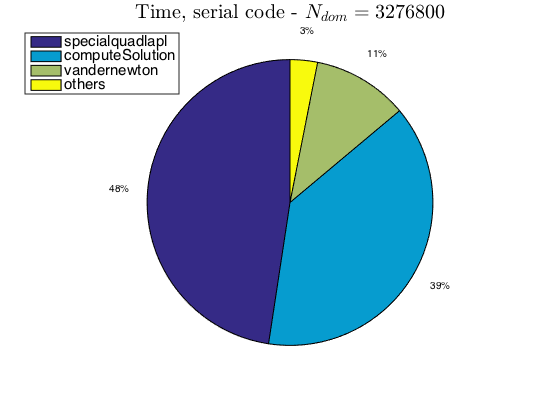
\includegraphics[width=0.49\textwidth]{Graphics/craypat_serial_batch10_time_pie.png}
    \end{center}
    \caption{Number of function calls and times for serial code $N_{dom} = 1600$, $N_{pan} = 20$.}
    \label{fig:batch10_serial_pie}
\end{figure} \\ \\
In comparison to the example with smaller $N_{dom}$, our cache utilization has now significantly approved among the costly functions. For all functions which make up the majority of the execution time all have D1 cache hit and miss ratios of $>99\%$. Also the D1+D2 cache hit,miss ratios are all $>99\%$. However, the D2 cache hit,miss ratios are worse, ranging from $55\%$ to $80.1\%$. 
\begin{table}[ht]
\begin{center}
    \begin{tabular}{ c | c | c | c | c }
        Function & D1 hit/miss (\%/\%) & D2 hit/miss & D1+D2 hit/miss & Time (\%) \\ \hline
        Total & $99.3/0.7$ & $67.8/32.2$ & $99.8/0.2$ & $100$ \\ 
        specialquadlapl & $99.1/0.9$ & $72.1/27.9$ & $99.7/0.3$ & $47.6$ \\
        computeSolution & $100/0$ & $80.1/19.9$ & $100/0$ & $38.5$ \\
        vandernewton & $99.4/0.6$ & $55/45$ & $99.7/0.3$ & $10.8$ \\
        IPmultR & $99.3/0.7$ & $68.8/31.2$ & $99.8/0.2$ & $1.6$
    \end{tabular}
    \caption{D1 and D2 cache hit and miss ratios for serial code, $N_{dom} = 3276800$. Data generated by CrayPAT.}
    \label{tab:batch4_serial_caches}
\end{center}
\end{table}  

\subsection*{Change boundary discretization}
Contrary to what we did previously, we will now see how the performance changes as we change $N_{pan}$ and keep $N_{dom}$ fixed. As a reference, we have selected a suitable $N_{dom} = 409 600$.



\todo[inline]{Define our testcase that we will test for different $N$.}
\todo[inline]{Analyze the serial code with e.g. Craypat and show timinigs etc.}
\todo[inline]{Define where we need to optimize our code}

\FloatBarrier
\section*{Speeding Up Our Code}
From the tests deducted on our serial code, we conclude that in the simulation cases we are interested in studying, i.e. for problems dominated by $N_{dom}$ over $N_{pan}$, it is most important to work with \textit{specquadlapl} and \textit{computeSolution} to achieve a speed-up. 

\subsection*{Improving the algorithm}
\todo[inline]{talk about cache misses here}
\todo[inline]{ collapse for loops computeSolution}

\subsection*{OpenMP}
\todo[inline]{Describe how we use OpenMP}
\todo[inline]{Show more timings for how this changes things}

\todo[inline]{computeSol all iterates take same time, good to set static}

\subsection*{MPI}
\todo[inline]{Describe how we use MPI}
\todo[inline]{SHow more timings}

\subsection*{Hybrid Method}
\todo[inline]{Should we use both OpenMP and MPI?}

\section*{Conclusions}
\todo[inline]{WHat is good, what is worth doing?}

\newpage
\begin{thebibliography}{99}
    \bibitem{ojalahelsing}
    Helsing, J. and Ojala, R., 2008. On the evaluation of layer potentials close to their sources. {\em Journal of Computational Physics}, 227(5), pp.2899-2921.
\end{thebibliography}

\newpage
\appendix
\section{Algorithms}
\label{sec:alg}
\begin{algorithm}[ht]
    \SetKwInOut{Input}{Input}
    \SetKwInOut{Output}{Output}

    \underline{Function solveDensity} $(z,zp,zpp,W, RHS)$\;
    \Input{Interface discretization points and derivatives: $z$, $zp$, $zpp$. Quadrature weights: $W$. Right hand side: $RHS$.}
    \Output{$\mu$}
    \For{go through all boundary points $i$} {
        \For{go through all boundary points $j$} {
            Fill dense matrix $A$: \\
                Elements $A_{ij} = \frac{1}{2\pi} W_j \Im\left\{ \frac{zp_j}{z_j - z_i} \right\}$. \\
                Elements $A_{ii} = \frac{1}{2} + \frac{1}{2\pi}W_i \Im\left\{ \frac{zpp_i}{2zp_i} \right\}$.
        }
    }
    Solve $A\mu=RHS$ with gmres.
    \caption{Computing complex density $\mu(z)$, for all $z\in\delta\Omega$.}
    \label{alg:solveDensity}
\end{algorithm}
\begin{algorithm}[ht]
    \SetKwInOut{Input}{Input}
    \SetKwInOut{Output}{Output}

    \underline{Function computeSolution} $(z,zp,\tau,W,\mu)$\;
    \Input{Interface discretization points and derivatives: $z$, $zp$. Domain discretization points $\tau$. Quadrature weights: $W$. Complex density $\mu$.}
    \Output{$u$}
    \For{go through all domain points $\tau_i$} {
        $u_i = 0$; \\
        \For{go through all boundary points $z_j$} {
            Compute velocity $u_i$: 
            $u_i = u_i + W_j\mu_j\Im\left\{ \frac{zp_j}{z_j-\tau_i} \right\}$;
        }
    }
    \caption{Computing solution to Laplace's equation $u$, for all $\tau\in\Omega$.}
    \label{alg:compU}
\end{algorithm}
\begin{algorithm}[ht]
    \SetKwInOut{Input}{Input}
    \SetKwInOut{Output}{Output}

    \underline{Function specialQuadrature} $(\tau,W, P_j, \mu, u)$\;
    \Input{Interface discretization points and derivatives: $z$, $zp$. Domain discretization points $\tau$. Quadrature weights: $W$. Complex density $\mu$. Solution $u$ computed with standard quadrature.}
    \Output{$u$}
    \For{go through all domain points $\tau_i$} {
        \For{go through all panels $P_j$} {
            Compute distance between $P_j$ and $\tau_i$, $d_{ij}$
            \If{$d_{ij} < TOL$} {
                Investigate this point-panel pair further: \\
                \begin{itemize}
                    \item Compute analytical solution to $p_0$.
                    \item Go through all panel points (16) and compute numerical approximation to $p_0$, $\hat{p}_0$.
                \end{itemize}
                \If{ $|p_0 - \hat{p}_0| > TOL$} {
                    Normal quadrature not sufficient to resolve this domain point.
                    Upsample to $32$-point Gauss-Legendre panel on $P_j$, $\tilde{z}_i$, and comupte $\hat{p}_0$ again. 
                    \If{ $|p_0 - \hat{p}_0| > TOL$} {
                        Upsample sufficient for resolution. Compute panel contribution anew by going throuhg points $\tilde{z}_i$. Remove panel contribution from 16-points G.-L. from $u$ and add new contribution from 32-points.
                    }
                    \Else {
                        Upsampling not sufficient. Apply special quadrature by computing all $p_k$ and interpolating, see REF. Then remove panel contribuiton from 16-points G.-L. from $u$ and add new solution. 
                    }
                }
                \Else {
                    Normal quadrature is sufficient. No recomputation needed.
                }
            }
        }

    }
    \caption{Computing solution to Laplace's equation $u$ with special quadrature, for all $\tau\in\Omega$.}
    \label{alg:specQ}
\end{algorithm}


\end{document}

